\documentclass{article}
\usepackage{tikz}
\usepackage{amsmath}
\usepackage{bm}
\usepackage{scalerel}
\usepackage{pgfplots}
\usepackage{mathpazo}
\pgfplotsset{width=7cm,compat=1.8}
\usetikzlibrary{patterns}
\usetikzlibrary{arrows,shapes,calc}
\usetikzlibrary{external}
\tikzset{external/system call={pdflatex \tikzexternalcheckshellescape -halt-on-error
        -interaction=batchmode -jobname "\image" "\texsource" && %  or ;
pdftops -eps "\image".pdf}}
\tikzexternalize


\begin{document}
	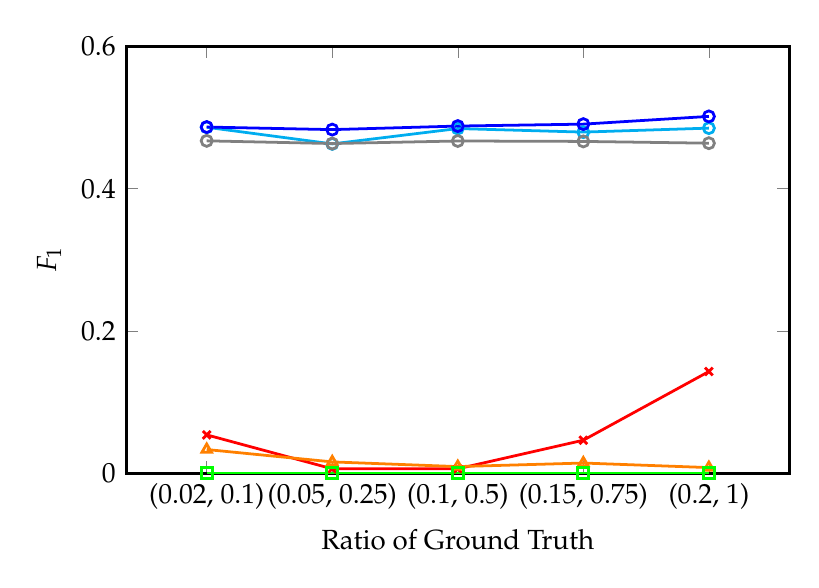
\begin{tikzpicture}
	\definecolor{lssfre}{HTML}{fccde5} %粉
	\definecolor{lssemb}{HTML}{bc80bd} %紫色
	\definecolor{lsscon}{HTML}{bebada} %淡紫色
	\definecolor{wj}{HTML}{fb8072} %橙色 深一点
	\definecolor{impr}{HTML}{80b1d3} %青蓝
	\definecolor{cs}{HTML}{fdb462} %橙色
	\definecolor{cset}{HTML}{b3de69}%绿色
	\definecolor{jsub}{HTML}{8dd3c7} %青绿
	\definecolor{sumrdf}{HTML}{ffffb3} %淡黄
	\definecolor{bsk}{HTML}{d9d9d9} %浅灰
	\definecolor{gflow}{HTML}{778899} %深灰色
	\definecolor{SB}{HTML}{F5F5DC}
	\definecolor{lc}{HTML}{FFFDD0}
	\definecolor{fire}{HTML}{FFE5B4}
	\definecolor{bo}{HTML}{E6E6FA}
	\definecolor{PINK}{HTML}{FFC0CB}
	\centering
	\begin{axis}[
	height=7cm, width=10cm,
	line width= 1pt,
	%enlarge y limits={value=.1,upper},
	ymin=0.0, ymax=0.6,
	%ymode=log,
	%log origin=infty,
	enlarge x limits=true,
	legend style={
		at={(0.5, 1.2)},
		anchor=north,
		legend columns=6
	},
	ylabel={$F_1$},
	%ytick={0.7, 0.8, 0.9, 1.0},
	%yticklabels={$0.7$, $0.8$, $0.9$, $1.0$},
	xmin=0.8, xmax = 5.2,
	xtick={1, 2, 3, 4, 5},
	xticklabels={(0.02, 0.1), (0.05, 0.25), (0.1, 0.5), (0.15, 0.75), (0.2, 1)},
	xlabel={Ratio of Ground Truth},
	%symbolic x coords={
	%	Facebook, Gowalla, WikiConflict, Google, DBLP, Berkstan, Youtube, Petster, Flickr,
	%Indochina },
	%xtick=data,
	]
	
	%MAML
 	\addplot [color=red,mark=x] coordinates {
	(1,0.0539)
	(2,0.0062)
	(3,0.0062)
	(4,0.0464)
	(5,0.143)
    };


	% inner product
 	\addplot [color=cyan,mark=o] coordinates {
	(1,0.4865)
	(2,0.4631)
	(3,0.4847)
	(4,0.4797)
	(5,0.4853)
    };
    
    % mlp
 	\addplot [color=blue,mark=o] coordinates {
	(1,0.4868)
	(2,0.4832)
	(3,0.4882)
	(4,0.4909)
	(5,0.5018)
	};
    
   	% gnn
 	\addplot [color=gray,mark=o] coordinates {
	(1,0.4674)
	(2,0.4636)
	(3,0.4672)
	(4,0.4666)
	(5,0.4641)
    };
    
    
    % FEATTRANS
 	\addplot [color=orange,mark=triangle] coordinates {
	(1,0.0333)
	(2,0.0159)
	(3,0.0093)
	(4,0.0143)
	(5,0.0079)
    };
    
    	% SUPERVISE
 	\addplot [color=green,mark=square] coordinates {
	(1,0)
	(2,0)
	(3,0)
	(4,0)
	(5,0)
    };
    
	\legend{
			%\large $\texttt{MAML}$,
		    %\large $\texttt{CGNP}$,
		    %\large $\texttt{CGNP\_MLP}$,
		    %\large $\texttt{CGNP\_GNN}$,
		    %\large $\texttt{FeatTrans}$,
		    %\large $\texttt{Supervised}$,
	        }
	\end{axis}
	\end{tikzpicture}
\end{document}